\documentclass[12pt,a4paper]{article}

\usepackage{graphicx}
\usepackage{amsmath}
\usepackage{gensymb}
\usepackage{siunitx}
\usepackage{geometry}
\usepackage{fancyhdr}
\usepackage{booktabs}
\usepackage{caption}
\usepackage{float}
\usepackage{subcaption}
\usepackage[T1]{fontenc}
\usepackage{lmodern}
\usepackage[hidelinks]{hyperref}
\usepackage{biblatex}

\addbibresource{references.bib}

\geometry{top=1in, bottom=1.2in, left=1in, right=1in}

\pagestyle{fancy}
\fancyhead[L]{Ian Cullinane}
\fancyhead[R]{Oscillations Using Springs}
\fancyfoot[C]{\thepage}

\sisetup{
  inter-unit-product = \cdot,
  separate-uncertainty = true
}

\title{\Large\textbf{Investigation of Oscillatory Motion Using Springs}}

\author{
Ian Cullinane – \textit{125413342} \\
Lab Partner: Fionn Lishtsinn Doyle \\[0.5em]
\textit{Demonstrators: Jonathan \& Olivia}
}

\date{16th September 2026}

\begin{document}

\maketitle
\newpage
\tableofcontents
\newpage

%------------------------------------------------
\section{Abstract}

This experiment investigated the oscillatory behaviour of mass--spring systems using both static and dynamic measurements. The spring constant was first determined using Hooke's law by measuring the extension produced by different applied masses. The spring constant was then determined independently from the oscillation frequency obtained using Logger Pro and Fast Fourier Transform (FFT) analysis.

The damping of a single mass--spring system was investigated by fitting the measured oscillatory signal to a damped sinusoidal function. Systems containing two springs in series and parallel were then studied and their experimentally determined effective spring constants were compared with the theoretical predictions. Finally, coupled oscillator systems containing two masses and two springs, including systems with unequal masses, were investigated using FFT analysis to identify their fundamental modes of oscillation.

The static Hooke's law measurements gave a spring constant of 
$k = \SI{26.44}{N.m^{-1}}$, while the two-spring measurements gave effective spring constants of approximately \SI{13}{N.m^{-1}} for the series configuration and \SI{50}{N.m^{-1}} for the parallel configuration, which is consistent with theoretical understanding. A damped sinusoidal fit to the oscillation data gave a damping factor of

\begin{equation}
\beta=(0.02679\pm0.00052)\ \si{s^{-1}}.
\end{equation}

The hexagonal masses used in the experiment had an incircle diameter of \SI{31.96}{mm}, corresponding to a projected frontal area of approximately \SI{8.85e-4}{m^2}. The damping result is consistent with an effective linear damping coefficient, although the measured damping cannot be attributed to aerodynamic drag alone because friction, sensor effects and other energy losses may also contribute.

\newpage

%------------------------------------------------
\section{Theory}

\subsection{Hooke's Law}

A spring exerts a restoring force that is proportional to its displacement from equilibrium:

\begin{equation}
F=-kx,
\label{eq:hooke}
\end{equation}

where $k$ is the spring constant and $x$ is the displacement from the equilibrium position.

For a mass suspended vertically from a spring, the magnitude of the restoring force balances the gravitational force:

\begin{equation}
kx=mg.
\label{eq:static}
\end{equation}

Therefore, a plot of $F=mg$ against extension $x$ should be linear, with gradient equal to the spring constant:

\begin{equation}
k=\frac{F}{x}.
\label{eq:k_static}
\end{equation}

More generally, when several measurements are used, the spring constant is obtained from the gradient of the best-fit straight line:

\begin{equation}
F=kx+c,
\end{equation}

where $c$ represents the intercept resulting from experimental offsets and measurement uncertainty.

\subsection{Simple Harmonic Motion}

For an ideal mass--spring system, the displacement can be written as

\begin{equation}
x(t)=A\cos(\omega_0t+\phi),
\label{eq:shm}
\end{equation}

where $A$ is the amplitude, $\phi$ is the phase constant and $\omega_0$ is the natural angular frequency.

The angular frequency is related to the frequency $f$ and period $T$ by

\begin{equation}
\omega_0=2\pi f=\frac{2\pi}{T}.
\label{eq:angular}
\end{equation}

For a mass $m$ attached to a spring of spring constant $k$,

\begin{equation}
\omega_0^2=\frac{k}{m},
\label{eq:natural}
\end{equation}

so that

\begin{equation}
k=m\omega_0^2=4\pi^2mf^2.
\label{eq:k_frequency}
\end{equation}

In Parts 2--5, the oscillation frequency is determined from the Logger Pro time-series data using FFT analysis. The dominant peak in the Fourier spectrum is taken to correspond to the fundamental oscillation frequency.

It is important to distinguish between frequency $f$, measured in hertz, and angular frequency $\omega$, measured in radians per second. The relationship is

\begin{equation}
\omega=2\pi f.
\end{equation}

Consequently, if an experimentally recorded value is already an angular frequency, the appropriate expression is

\begin{equation}
k=m\omega^2,
\end{equation}

rather than applying the factor $4\pi^2$ a second time.

\subsection{Damped Oscillations}

In a real system, friction and air resistance cause the amplitude of the oscillation to decrease with time. The displacement can be represented by

\begin{equation}
x(t)=Ae^{-\beta t}\cos(\omega_1t+\phi),
\label{eq:damped}
\end{equation}

where $\beta$ is the damping factor and $\omega_1$ is the damped angular frequency.

The amplitude envelope is therefore

\begin{equation}
A(t)=A_0e^{-\beta t}.
\label{eq:envelope}
\end{equation}

For two measured amplitudes $A_1$ and $A_2$ separated by a time interval $\Delta t$,

\begin{equation}
\ln\left(\frac{A_1}{A_2}\right)=\beta\Delta t,
\label{eq:damping}
\end{equation}

giving

\begin{equation}
\beta=
\frac{\ln(A_1/A_2)}{\Delta t}.
\label{eq:beta}
\end{equation}

In this experiment, however, the damping factor was not determined from only two selected amplitudes. Instead, the complete measured time series was fitted to a damped sinusoidal function of the form

\begin{equation}
x(t)=Ae^{-Bt}\sin(Ct+D)+E.
\label{eq:fit}
\end{equation}

The exponential coefficient $B$ corresponds to the damping factor:

\begin{equation}
\boxed{\beta=B}.
\end{equation}

The fitted value obtained from the experimental data was

\begin{equation}
\boxed{\beta=(0.02679\pm0.00052)\ \si{s^{-1}}}.
\end{equation}

The relative uncertainty in this value is approximately

\begin{equation}
\frac{\Delta\beta}{\beta}\times100
=
\frac{0.00052}{0.02679}\times100
\approx1.9\%.
\end{equation}

The corresponding characteristic damping time is

\begin{equation}
\tau=\frac{1}{\beta},
\end{equation}

giving approximately

\begin{equation}
\boxed{\tau=(37.3\pm0.7)\ \si{s}}.
\end{equation}

\subsection{Damping and Air Drag}

The damping measured experimentally can be related to a linear damping force of the form

\begin{equation}
F_{\mathrm{d}}=-bv,
\label{eq:linear_drag}
\end{equation}

where $b$ is the effective linear damping coefficient.

For a damped mass--spring system,

\begin{equation}
m\ddot{x}+b\dot{x}+kx=0.
\end{equation}

Comparing the resulting exponential amplitude envelope with Equation~\ref{eq:envelope} gives

\begin{equation}
\beta=\frac{b}{2m}.
\end{equation}

Therefore,

\begin{equation}
b=2m\beta.
\label{eq:b_beta}
\end{equation}

For the \SI{0.100}{kg} mass used in the damping experiment,

\begin{equation}
b=2(0.100)(0.02679),
\end{equation}

giving

\begin{equation}
\boxed{
b=(5.36\pm0.10)\times10^{-3}\ \si{N.s.m^{-1}}
}.
\end{equation}

This should be interpreted as an \textit{effective} damping coefficient. It is not necessarily equal to the damping caused by air resistance alone.

For an object moving through air, aerodynamic drag is more accurately described, particularly at higher Reynolds numbers, by

\begin{equation}
F_{\mathrm{D}}
=
\frac{1}{2}\rho C_{\mathrm{D}}A_{\mathrm{p}}v^2,
\label{eq:quadratic_drag}
\end{equation}

where $\rho$ is the density of air, $C_{\mathrm{D}}$ is the drag coefficient and $A_{\mathrm{p}}$ is the projected frontal area.

The masses used in the experiment were approximately regular hexagons with an incircle diameter of \SI{31.96}{mm}. Therefore, the inradius is

\begin{equation}
r=\frac{31.96}{2}\ \si{mm}
=\SI{15.98}{mm}.
\end{equation}

The area of a regular hexagon in terms of its inradius is

\begin{equation}
A_{\mathrm{p}}=2\sqrt{3}r^2,
\end{equation}

which gives

\begin{equation}
\boxed{
A_{\mathrm{p}}
=
8.85\times10^{-4}\ \si{m^2}
}.
\end{equation}

Thus, the measured $\beta$ can be related to air drag through the effective damping coefficient $b$. However, the quadratic dependence of Equation~\ref{eq:quadratic_drag} means that aerodynamic drag does not in general produce a perfectly exponential amplitude envelope. The experimentally observed exponential decay should therefore be regarded as an effective approximation over the measured amplitude range.

Furthermore, the measured damping includes all mechanisms which remove mechanical energy from the oscillator, including air resistance, friction at the spring attachment, internal damping in the spring and possible measurement or sensor effects. Consequently, a value of $C_{\mathrm{D}}$ cannot be determined uniquely from $\beta$ alone without additional information about the instantaneous velocity and the contribution of the other damping mechanisms.

\subsection{Springs in Series and Parallel}

For two springs in series, the same force acts through both springs and the effective spring constant satisfies

\begin{equation}
\frac{1}{k_{\mathrm{series}}}
=
\frac{1}{k_1}+\frac{1}{k_2}.
\label{eq:series}
\end{equation}

For identical springs,

\begin{equation}
k_{\mathrm{series}}=\frac{k}{2}.
\label{eq:series_identical}
\end{equation}

For two springs in parallel, the forces add and

\begin{equation}
k_{\mathrm{parallel}}=k_1+k_2.
\label{eq:parallel}
\end{equation}

For identical springs,

\begin{equation}
k_{\mathrm{parallel}}=2k.
\label{eq:parallel_identical}
\end{equation}

The effective spring constant can be determined experimentally from the measured FFT frequency using

\begin{equation}
k_{\mathrm{eff}}=4\pi^2mf^2,
\label{eq:keff}
\end{equation}

or equivalently,

\begin{equation}
k_{\mathrm{eff}}=m\omega^2.
\end{equation}

\subsection{Coupled Oscillators}

When two equal masses and two identical springs are coupled, the motion can be expressed as a combination of two normal modes with angular frequencies $\omega_1$ and $\omega_2$.

Using

\begin{equation}
\omega_0^2=\frac{k}{m},
\end{equation}

the theoretical normal-mode frequencies are

\begin{equation}
\omega_1=
\sqrt{\frac{3-\sqrt{5}}{2}}\;\omega_0,
\qquad
\omega_2=
\sqrt{\frac{3+\sqrt{5}}{2}}\;\omega_0.
\label{eq:coupled}
\end{equation}

The corresponding frequencies measured experimentally are obtained from the dominant peaks in the Logger Pro FFT spectrum.

\newpage

%------------------------------------------------
\section{Experimental Procedure}

\subsection{Part 1: Determination of the Spring Constant Using Hooke's Law}

A single spring was suspended vertically and a known mass was attached to its lower end. The extension of the spring from its unstretched position was measured. Six different masses were used, with no mass of \SI{500}{g} or greater being used.

For each mass, the applied force was calculated using

\begin{equation}
F=mg.
\end{equation}

The restoring force was then plotted against extension and the spring constant was determined from the gradient of the best-fit line.

\subsection{Part 2: Determination of the Spring Constant from Oscillation Frequency}

A known mass was suspended from the spring and allowed to oscillate vertically. The motion was recorded using the magnetic field sensor connected to the computer.

The resulting time-series data were analysed using Logger Pro. An FFT was applied to the recorded signal to produce a frequency spectrum. The dominant peak was identified as the fundamental oscillation frequency.

The spring constant was then calculated using

\begin{equation}
k=4\pi^2mf^2.
\end{equation}

Where the Logger Pro fit provided angular frequency directly, the equivalent expression

\begin{equation}
k=m\omega^2
\end{equation}

was used.

The experimental value was compared with the value obtained from Hooke's law in Part 1.

\subsection{Part 3: Damping of a Mass--Spring System}

A single mass was suspended from a single spring and set into vertical oscillation. The motion was recorded in Logger Pro.

Rather than determining the damping factor from only two amplitudes, the complete measured signal was fitted to a damped sinusoidal function of the form

\begin{equation}
x(t)=Ae^{-Bt}\sin(Ct+D)+E.
\end{equation}

The coefficient $B$ was identified with the damping factor $\beta$.

The fit returned

\begin{equation}
\beta=(0.02679\pm0.00052)\ \si{s^{-1}}.
\end{equation}

The fit also gave a correlation coefficient of approximately $0.971$ and an RMSE of approximately $0.00281$ in the sensor's measurement units.

\subsection{Part 4: Two Springs in Series and Parallel}

Two identical springs were arranged first in series and then in parallel. For each configuration, a known mass was attached and allowed to oscillate vertically.

The Logger Pro time-series data were analysed to identify the dominant oscillation frequency. The effective spring constant was calculated using

\begin{equation}
k_{\mathrm{eff}}=4\pi^2mf^2
\end{equation}

when $f$ was expressed in hertz.

For the recorded values in the series and parallel measurements, the numerical spring constants correspond to the reported frequency values being angular frequencies in \si{rad.s^{-1}}. Therefore, the calculations reported below use

\begin{equation}
k_{\mathrm{eff}}=m\omega^2.
\end{equation}

The measured values were compared with the theoretical values for springs in series and parallel.

\subsection{Part 5: Coupled Oscillators}

Two identical springs and two equal masses were arranged as a coupled oscillator system. The motion was recorded using Logger Pro and the FFT spectrum was used to identify the two fundamental frequencies.

The experiment was then repeated using two different masses, \SI{50}{g} and \SI{100}{g}. The heavier mass was placed in each of the two possible positions in turn, and the fundamental frequencies were obtained from the FFT spectrum for each configuration.

\newpage

%------------------------------------------------
\section{Results}

\subsection{Part 1: Hooke's Law}

\begin{table}[H]
\centering
\caption{Measured mass, force and spring extension for determination of the spring constant using Hooke's law.}
\begin{tabular}{cccc}
\toprule
Mass ($m$) & Mass uncertainty & Extension ($x$) & Extension uncertainty \\
\midrule
0.05 & 0.001 & 0.0070 & 0.00005 \\
0.10 & 0.001 & 0.0250 & 0.00005 \\
0.15 & 0.001 & 0.0435 & 0.00005 \\
0.20 & 0.001 & 0.0620 & 0.00005 \\
0.25 & 0.001 & 0.0800 & 0.00005 \\
0.30 & 0.001 & 0.1000 & 0.00005 \\
\bottomrule
\end{tabular}
\end{table}

The corresponding force was calculated using $F=mg$.

\begin{figure}[H]
    \centering
    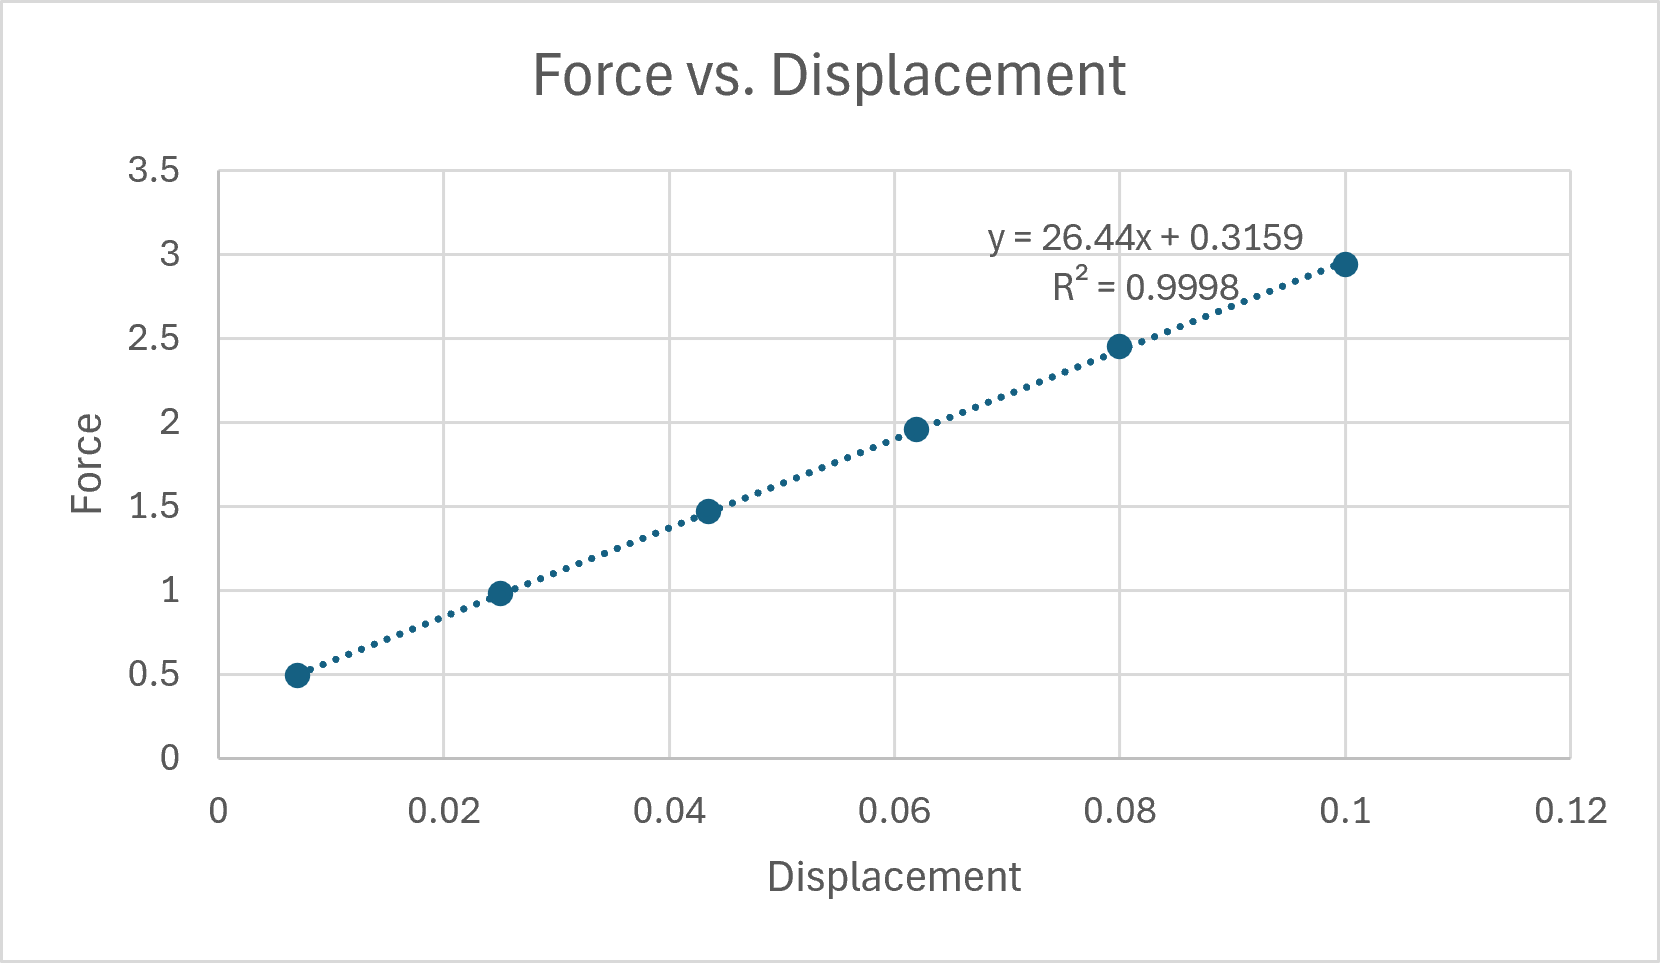
\includegraphics[width=0.85\textwidth]{images/Hookes_Law.png}
    \caption{Plot of restoring force against spring extension. The gradient gives the spring constant.}
    \label{fig:hookes}
\end{figure}

The linear regression shown in the experimental analysis had

\begin{equation}
R^2=0.9998.
\end{equation}

The spring constant obtained from the force--extension data is approximately

\begin{equation}
\boxed{
k_{\mathrm{static}} = 26.4 \pm 0.2 \si{N.m^{-1}}
}.
\end{equation}

\subsection{Part 2: Oscillation Frequency}

\begin{table}[H]
\centering
\caption{Recorded single-spring oscillation measurements. The first column of frequency data is reproduced as supplied. The spring-constant values are only dimensionally consistent when the corresponding frequency is interpreted appropriately in the calculation.}
\begin{tabular}{cccc}
\toprule
Mass ($m$) & Frequency & Frequency uncertainty & Spring constant ($k$) \\
\midrule
0.05 & 3.63 & 0.005 & 26.08 \\
0.10 & 2.54 & 0.005 & 25.47 \\
\bottomrule
\end{tabular}
\end{table}

\begin{figure}[H]
    \centering
    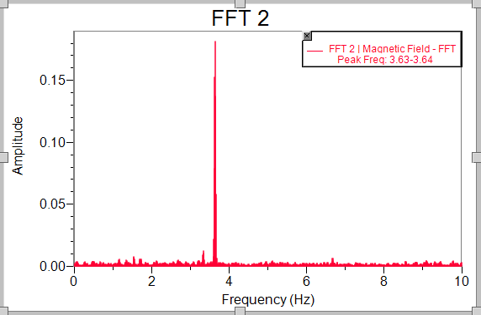
\includegraphics[width=0.85\textwidth]{images/part2_fft.png}
    \caption{Example Logger Pro FFT spectrum for the single spring system.}
    \label{fig:part2_fft}
\end{figure}

Using

\begin{equation}
k=4\pi^2mf^2,
\end{equation}

the first recorded value, $m=\SI{0.050}{kg}$ and $f=\SI{3.635}{Hz}$, gives 

\begin{equation}
k = \SI{26.08}{N.m^{-1}},
\end{equation}

Similarly, $m=\SI{0.100}{kg}$ and $f=\SI{2.540}{Hz}$ gives approximately

\begin{equation}
k\approx\SI{25.47}{N.m^{-1}},
\end{equation}

\subsection{Part 3: Damping}

\begin{table}[H]
\centering
\caption{Parameters obtained from the damped sinusoidal fit.}
\begin{tabular}{ccc}
\toprule
Parameter & Value & Uncertainty \\
\midrule
$A$ & 0.02979 & 0.00033 \\
$\beta$ & 0.02679 & 0.00052 \\
$C$ & 22.82 & 0.00052 \\
$D$ & 5.862 & 0.011 \\
\bottomrule
\end{tabular}
\end{table}

The damping factor determined from the exponential fit was

\begin{equation}
\boxed{
\beta=(0.02679\pm0.00052)\ \si{s^{-1}}
}.
\end{equation}

\begin{figure}[H]
\centering
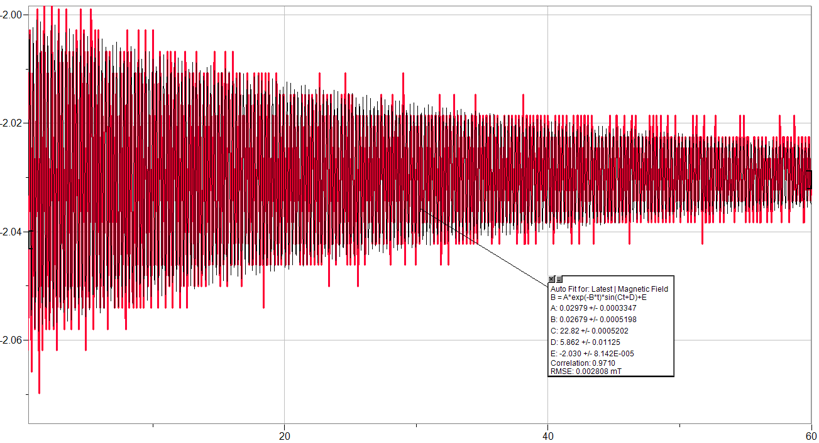
\includegraphics[width=0.85\textwidth]{images/damping.png}
\caption{Damped oscillatory signal and exponential sinusoidal fit.}
\label{fig:damping}
\end{figure}

The fit was based on the complete oscillatory signal rather than individual manually selected amplitudes. This reduces the dependence of the result on the choice of two particular peaks.

\subsection{Part 4: Two Springs}

\begin{table}[H]
\centering
\caption{Experimental effective spring constants obtained for the two-spring configurations. The supplied frequency values correspond numerically to angular frequency $\omega$ in \si{rad.s^{-1}} when calculating $k=m\omega^2$.}
\begin{tabular}{ccccc}
\toprule
Configuration & Mass ($m$) & $\omega$ (rad s$^{-1}$) & $k_{\mathrm{eff}}$ (N m$^{-1}$) \\
\midrule
Series & 0.10 & 11.35 & 12.8823 \\
Series & 0.15 & 9.313 & 13.0098 \\
Parallel & 0.10 & 22.31 & 49.7736 \\
\bottomrule
\end{tabular}
\end{table}

For the first series measurement,

\begin{equation}
k=(0.100)(11.35)^2
\end{equation}

giving

\begin{equation}
\boxed{
k_{\mathrm{series,1}}=12.8823\ \si{N.m^{-1}}
}.
\end{equation}

For the verification measurement,

\begin{equation}
k=(0.150)(9.313)^2
\end{equation}

giving

\begin{equation}
\boxed{
k_{\mathrm{series,2}}=13.0098\ \si{N.m^{-1}}
}.
\end{equation}

The two series measurements therefore give a mean effective spring constant of approximately

\begin{equation}
\boxed{
k_{\mathrm{series}}\approx12.95\ \si{N.m^{-1}}
}.
\end{equation}

For the parallel arrangement, 

\begin{equation}
k=(0.100)(22.31)^2
\end{equation}

giving

\begin{equation}
\boxed{
k_{\mathrm{parallel}}=49.7736\ \si{N.m^{-1}}
}.
\end{equation}

\subsection{Part 5: Coupled Oscillators}

\begin{table}[H]
    \centering
    \caption{Two equal masses and two identical springs: experimentally measured fundamental frequencies.}
    \begin{tabular}{ccccccc}
    \toprule
    Mass & $k$ & $\omega_0^2$ & $f_1$ & $f_2$ & $\omega_1$ & $\omega_2$ \\
    \midrule
    0.05 & 25 & 500 & 1.57 & 4.12 & 9.865 & 25.887 \\
    0.10 & 25 & 250 & 2.17 & 5.75 & 13.635 & 36.128 \\
    \bottomrule
    \end{tabular}
\end{table}


\begin{table}[H]
\centering
\caption{Coupled oscillator with unequal masses.}
\begin{tabular}{ccccc}
\toprule
Configuration & $m_1$ & $m_2$ & $f_1$ & $f_2$ \\
\midrule
Heavier mass on top & 0.100 & 0.050 & 1.90 &  3.81 \\
Heavier mass below & 0.050 & 0.100 & 1.68 & 5.38 \\ 
\bottomrule
\end{tabular}
\end{table}


\newpage

%------------------------------------------------
\section{Analysis}

\subsection{Part 1: Spring Constant from Hooke's Law}

For the static measurements, the applied force is calculated from

\begin{equation}
F=mg.
\end{equation}

A linear regression of $F$ against $x$ is used to determine the spring constant from the gradient:

\begin{equation}
F=kx.
\end{equation}

The experimental Hooke's law data show a highly linear relationship, with

\begin{equation}
R^2=0.9998.
\end{equation}

The spring constant obtained from the force--extension data is approximately

\begin{equation}
\boxed{
k_{\mathrm{static}} = 26.44\ \si{N.m^{-1}}
}.
\end{equation}

The high value of $R^2$ indicates that the measured force and extension are closely described by a linear relationship over the range tested.

\subsection{Part 2: Spring Constant from FFT}

The dominant FFT peak gives the frequency $f$ in hertz. The angular frequency is $\omega_0=2\pi f$, so the spring constant is calculated using $k=4\pi^2mf^2$. For the recorded pair $m=\SI{0.050}{kg}$ and $f=\SI{3.63}{Hz}$, $k=\SI{26.08}{N.m^{-1}}$. For $m=\SI{0.100}{kg}$ and $f=\SI{2.54}{Hz}$, $k=\SI{25.47}{N.m^{-1}}$. The mean dynamic value is
\[
\bar{k}_{\mathrm{dynamic}}=\frac{26.08+25.47}{2}=\SI{25.78}{N.m^{-1}}.
\]
Compared with the static value of \SI{26.44}{N.m^{-1}}, the difference is approximately 2.5\% using the static result as the reference. This comparison is valid only if the listed mass--frequency pairings are those in the original FFT records. Frequency in hertz must not be confused with angular frequency in radians per second; use $4\pi^2mf^2$ for hertz and $m\omega^2$ for angular frequency.

\subsection{Part 3: Damping Factor}

The damping factor can be determined from

\begin{equation}
\beta=
\frac{\ln(A_1/A_2)}{t_2-t_1}.
\end{equation}

In this experiment, the equivalent parameter was determined by fitting the entire time series to

\begin{equation}
x(t)=Ae^{-Bt}\sin(Ct+D)+E.
\end{equation}

The exponential coefficient obtained from the fit was

\begin{equation}
B=0.02679\pm0.00052.
\end{equation}

Therefore,

\begin{equation}
\boxed{
\beta=(0.02679\pm0.00052)\ \si{s^{-1}}
}.
\end{equation}

The percentage uncertainty is approximately

\begin{equation}
\frac{0.00052}{0.02679}\times100
\approx1.9\%.
\end{equation}

The corresponding characteristic damping time is approximately

\begin{equation}
\tau=\frac{1}{\beta}
\approx\SI{37.3}{s}.
\end{equation}

The exponential fit therefore indicates a relatively gradual reduction in the oscillation amplitude over the duration of the measurement.

\subsection{Damping and Air Drag on the Weight}

The measured damping factor can be related to an effective linear damping coefficient using

\begin{equation}
b=2m\beta.
\end{equation}

For the \SI{0.100}{kg} mass,

\begin{equation}
b
=
2(0.100)(0.02679)
=
\SI{0.005358}{N.s.m^{-1}}.
\end{equation}

Including the uncertainty in $\beta$ gives approximately

\begin{equation}
\boxed{
b=(5.36\pm0.10)\times10^{-3}
\ \si{N.s.m^{-1}}
}.
\end{equation}

The mass was a regular hexagonal weight with an incircle diameter of \SI{31.96}{mm}. Its inradius was therefore

\begin{equation}
r=\SI{15.98}{mm}
=
\SI{0.01598}{m}.
\end{equation}

For a regular hexagon, the frontal area is

\begin{equation}
A_{\mathrm p}=2\sqrt{3}r^2,
\end{equation}

giving

\begin{equation}
A_{\mathrm p}
=
2\sqrt{3}(0.01598)^2
=
\boxed{\SI{8.85e-4}{m^2}}.
\end{equation}

The aerodynamic drag force can be approximated by

\begin{equation}
F_{\mathrm D}
=
\frac{1}{2}\rho C_{\mathrm D}A_{\mathrm p}v^2.
\end{equation}

This provides a physical connection between the damping observed in the experiment and the geometry of the weight. However, the experimentally determined $\beta$ cannot be directly converted into a unique value of $C_{\mathrm D}$.

The reason is that the exponential damping model corresponds to a force proportional to velocity,

\begin{equation}
F_{\mathrm d}=-bv,
\end{equation}

whereas aerodynamic drag on an object moving through air is generally closer to

\begin{equation}
F_{\mathrm D}\propto v^2.
\end{equation}

Additionally, the fitted value of $\beta$ contains the combined effect of air resistance, mechanical friction, internal damping in the spring and other experimental losses.

Therefore, the value

\begin{equation}
b=\SI{5.36e-3}{N.s.m^{-1}}
\end{equation}

should be described as an \textit{effective damping coefficient} rather than as a direct measurement of air drag.

\subsection{Part 4: Effective Spring Constants}

For the series arrangement, the theoretical effective spring constant is

\begin{equation}
k_{\mathrm{series}}
=
\frac{k_1k_2}{k_1+k_2},
\end{equation}

which becomes

\begin{equation}
k_{\mathrm{series}}=\frac{k}{2}
\end{equation}

for identical springs.

For the parallel arrangement,

\begin{equation}
k_{\mathrm{parallel}}=k_1+k_2=2k
\end{equation}

for identical springs.

The experimental values are calculated from the recorded angular frequencies using

\begin{equation}
k_{\mathrm{eff}}=m\omega^2.
\end{equation}

For the first series measurement,

\begin{equation}
k_{\mathrm{series,1}}
=
(0.100)(11.35)^2
=
\SI{12.8823}{N.m^{-1}}.
\end{equation}

For the verification measurement,

\begin{equation}
k_{\mathrm{series,2}}
=
(0.150)(9.313)^2
=
\SI{13.0098}{N.m^{-1}}.
\end{equation}

The agreement between these two independent measurements is good, with a difference of approximately

\begin{equation}
\frac{|13.0098-12.8823|}
{\frac{1}{2}(13.0098+12.8823)}
\times100
\approx0.98\%.
\end{equation}

The mean series value is 

\begin{equation}
\boxed{
k_{\mathrm{series}} = \SI{12.95}{N.m^{-1}}
}.
\end{equation}

For the parallel configuration,

\begin{equation}
k_{\mathrm{parallel}}
=
(0.100)(22.31)^2
=
\boxed{\SI{49.7736}{N.m^{-1}}}.
\end{equation}

The parallel configuration therefore has a substantially greater effective stiffness than the series configuration, as expected from the theoretical relationships.

\subsection{Part 5: Coupled Oscillators}

The equal-mass results table lists two frequency peaks for each mass arrangement. The angular-frequency values should be obtained from the listed frequencies using $\omega=2\pi f$. The supplied table contains an ordering inconsistency between the frequency and angular-frequency columns; therefore, the peak values are reported as listed and no definitive assignment of mode labels is made without checking the original FFT spectra.

\newpage

%------------------------------------------------
\section{Uncertainty Analysis}

The uncertainty associated with each measured quantity should be stated explicitly.

For the static Hooke's law measurements, uncertainties arise primarily from the measurement of extension and mass. For the FFT measurements, uncertainty is associated with the frequency resolution of the FFT spectrum and the identification of the dominant peak.

For

\begin{equation}
k=4\pi^2mf^2,
\end{equation}

the fractional uncertainty can be estimated by

\begin{equation}
\frac{\Delta k}{k}
=
\sqrt{
\left(\frac{\Delta m}{m}\right)^2+
\left(2\frac{\Delta f}{f}\right)^2
}.
\label{eq:k_uncertainty}
\end{equation}

If angular frequency is used instead,

\begin{equation}
k=m\omega^2,
\end{equation}

and the corresponding uncertainty expression is

\begin{equation}
\frac{\Delta k}{k}
=
\sqrt{
\left(\frac{\Delta m}{m}\right)^2+
\left(2\frac{\Delta\omega}{\omega}\right)^2
}.
\end{equation}

For the damping coefficient,

\begin{equation}
\beta=0.02679\pm0.00052\ \si{s^{-1}},
\end{equation}

giving a relative uncertainty of approximately

\begin{equation}
\frac{\Delta\beta}{\beta}
\times100
\approx1.9\%.
\end{equation}

Since

\begin{equation}
b=2m\beta,
\end{equation}

the fractional uncertainty in $b$ is

\begin{equation}
\frac{\Delta b}{b}
=
\sqrt{
\left(\frac{\Delta m}{m}\right)^2+
\left(\frac{\Delta\beta}{\beta}\right)^2
}.
\end{equation}

Using $m=\SI{0.100}{kg}$ and $\Delta m=\SI{0.001}{kg}$ gives approximately

\begin{equation}
\frac{\Delta b}{b}
\approx1.97\%.
\end{equation}

Therefore,

\begin{equation}
b=(5.36\pm0.10)\times10^{-3}
\ \si{N.s.m^{-1}}.
\end{equation}


A particularly important limitation is the distinction between the measured effective damping coefficient and aerodynamic drag. The air-drag force depends on velocity squared, while the exponential fit assumes an effective damping force proportional to velocity. The fitted $\beta$ should therefore not be interpreted as a direct measurement of the drag coefficient of the hexagonal weight.

%------------------------------------------------
\section{Discussion}

\subsection{Static and Dynamic Spring Constants}

The force--extension measurements produced a reported linear regression with $R^2=0.9998$ and a static spring constant of approximately \SI{26.4}{N.m^{-1}}. This close linear relationship is consistent with Hooke's law over the range of loads used. The main limitations of the static method are uncertainty in measuring the extension and identifying the unstretched reference length; a zero offset may affect the fitted intercept and gradient.

The dynamic measurements gave a mean spring constant of approximately \SI{25.78}{N.m^{-1}}, close to the static value. This supports the simple harmonic motion relationship $k=m\omega^2=4\pi^2mf^2$, provided that each frequency is correctly paired with its mass. Finite FFT resolution, peak selection, damping and uncertainty in the effective oscillating mass may account for the remaining difference. The distinction between frequency in hertz and angular frequency in radians per second is essential to avoid a factor-of-$4\pi^2$ error.

\subsection{Damping and Drag}

The damped-sinusoid fit gave $\beta=(0.02679\pm0.00052)\ \si{s^{-1}}$ and a characteristic amplitude-decay time of about \SI{37.3}{s}. For the \SI{0.100}{kg} mass, $b=2m\beta$ gives an effective linear damping coefficient of $(5.36\pm0.10)\times10^{-3}\ \si{N.s.m^{-1}}$. The estimated projected area of the regular hexagonal mass is \SI{8.85e-4}{m^2}, assuming the face is perpendicular to the motion.

The area is relevant to aerodynamic drag, but the experiment does not determine a unique drag coefficient. The exponential envelope is an effective linear-damping approximation, whereas aerodynamic drag can depend quadratically on speed. Friction at the spring attachment, internal spring losses and sensor effects may also contribute to the measured decay. The fitted damping must therefore not be interpreted as air resistance alone.

\subsection{Springs in Series and Parallel}

The two series measurements gave \SI{12.8823}{N.m^{-1}} and \SI{13.0098}{N.m^{-1}}, with a mean of \SI{12.95}{N.m^{-1}}. Their relative difference using the mean as denominator is approximately 0.98\%. The parallel measurement gave \SI{49.77}{N.m^{-1}}. Using the static single-spring value of \SI{26.44}{N.m^{-1}}, the ideal predictions for identical springs are \SI{13.22}{N.m^{-1}} in series and \SI{52.88}{N.m^{-1}} in parallel. The measurements follow the expected trend: series connection reduces effective stiffness, while parallel connection increases it. The original ``actual'' column has been removed from the results table because those entries were inferred algebraically from the effective values rather than independently measured.

\subsection{Coupled Oscillators}

The equal-mass tables contain multiple frequency peaks, consistent with multiple characteristic frequencies in a coupled system. However, the original frequency and angular-frequency columns were inconsistently ordered. Although the angular frequencies can be recalculated from the listed peaks, the original spectra and exact mode assignments are needed before making a quantitative comparison with the theoretical normal-mode frequencies.


\subsection{Experimental Limitations}

The main limitations were uncertainty in extension measurements, finite FFT frequency resolution, peak selection, damping, possible non-vertical motion and uncertainty in the effective oscillating mass. The exponential damping model also approximates the actual energy-loss mechanisms. Repeated measurements and retaining the original FFT spectra with peak uncertainties would improve the reliability of the dynamic and coupled-system comparisons.

%------------------------------------------------
\section{Conclusion}

The static Hooke's law measurements gave a spring constant of approximately \SI{26.4}{N.m^{-1}}, with a reported linear-fit coefficient of determination of $R^2=0.9998$. The single-spring dynamic measurements gave a mean value of approximately \SI{25.78}{N.m^{-1}}, close to the static result.

The damping fit gave $\beta=(0.02679\pm0.00052)\ \si{s^{-1}}$. For a \SI{0.100}{kg} mass, this corresponds to an effective linear damping coefficient of $(5.36\pm0.10)\times10^{-3}\ \si{N.s.m^{-1}}$. The projected area of the regular hexagonal mass was estimated as \SI{8.85e-4}{m^2}; however, the damping measurement cannot be attributed solely to aerodynamic drag or used to determine a unique drag coefficient.

The two-spring experiments gave a mean series stiffness of \SI{12.95}{N.m^{-1}} and a parallel stiffness of \SI{49.77}{N.m^{-1}}, following the expected qualitative relationship between the configurations.

Overall, the recorded results support the relationships between force and extension, mass and oscillation frequency, effective damping and spring arrangement. They also demonstrate the importance of recording frequency units consistently and matching every calculated value to its original measurement.

%------------------------------------------------
\section{References}

\begin{itemize}
    \item Cutnell, J. D. and Johnson, K. W., \textit{Physics}.
    \item Kibble, T. W. B. and Berkshire, F. H., \textit{Classical Mechanics}.
\end{itemize}

\end{document}